\documentclass{beamer}
\usetheme{Pittsburgh}

\usepackage[utf8]{inputenc}
\usepackage[procnames]{listings}
\usepackage{listings}
\usepackage{graphicx}
%\usepackage[toc,page]{appendix}
\usepackage{caption}
\usepackage{hyperref}
\usepackage{color}
\usepackage{ulem}
%\usepackage{minted}

%Python
\definecolor{keywords}{RGB}{255,0,90}
\definecolor{comments}{RGB}{0,0,113}
\definecolor{red}{RGB}{160,0,0}
\definecolor{green}{RGB}{0,150,0}
\lstset{language=Python, 
    basicstyle=\ttfamily\scriptsize, 
    keywordstyle=\color{keywords},
    commentstyle=\color{comments},
    stringstyle=\color{red},
    identifierstyle=\color{green},
    procnamekeys={def,class},
    breaklines=true,
    columns=fullflexible,
    %Numbering and Tabs
    %numbers=left,
    %tabsize=4,
    %showspaces=false,
    %showstringspaces=false
    }

\begin{document}

\title{Python 2.7.6}
\subtitle{Threading and Networking}
\author{
  Mallick, Arka\\
  Naazare, Menaka \\
  Nair, Deebul\\
  Quignon, Christophe \\
} 
\institute{Hochschule Bonn Rhein Sieg}
\date{\today}

\begin{frame}
\titlepage
\end{frame}

%Chris
\begin{frame}[fragile]
\frametitle{Thread}
Withs thread, multiple parts of the program can run interleaved. Threads are linked to their program (process) and share memory and state with it.
The threads will not leave the CPU of the program and thus will not decrease the runtime of your program. But they are executed in "parallel" (more correct: interleaved), which may come in handy.


\begin{lstlisting}[language=Python]
import threading

thread.start_new_thread(function, args[, kwargs])

thread.start()
thread.run()
thread.join([timeout])
thread.is_alive()
\end{lstlisting}
\end{frame}

\begin{frame}[fragile]
\frametitle{Processes}
A process is an own instance of a programm. They are totally independent and thus can exploit multiple CPUs. They may communicate. 

\begin{lstlisting}[language=Python]
from multiprocessing import Process, Pool

pool = Pool(processes=8)#Number of Cores or more
result = pool.apply_async(function, [args])

#same as Threads
process.pid
process.authkey
process.terminate()
\end{lstlisting}
\end{frame}


%Arka
\begin{frame}[fragile]
\frametitle{Sharing Information Between Threads}
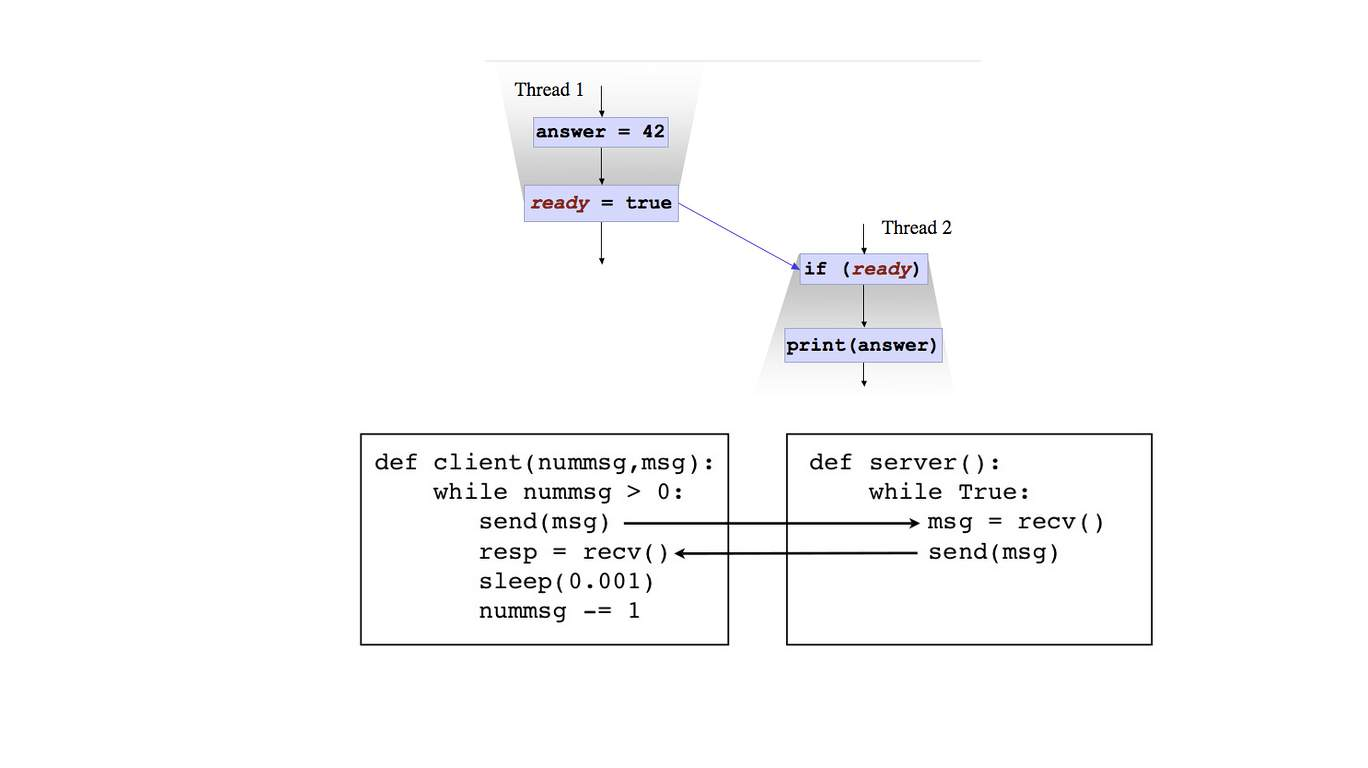
\includegraphics[scale=0.5]{datashare.jpg}
\end{frame}


%Menaka
\begin{frame}[fragile]
\frametitle{Thread Synchronization}

In order to avoid conflicts when more than one thread needs to access a single variable or other resource, threads have to be synchronized. \\
 
So, How is it done in python? \\
\begin{enumerate}
 \item Lock
 \item Rlocks
 \item Semaphores
 \item Events
 \item Conditions
 \item Queues
\end{enumerate}
\end{frame}


%Deebul
\begin{frame}[fragile]
\frametitle{Inter-Process Communication and Networking}
{Process can "talk" to each other using the following methods :}
\begin{enumerate}
 \item Files
 \item Pipes
 \item Signals
 \item Named Pipes
 \item Shared Memory
 \item Network Sockets
 \item RPC, XML-RPC
\end{enumerate}

\end{frame}

\begin{frame}[fragile]
\frametitle{ Networking}
{Sockets}
\begin{enumerate}
 \item Programming abstraction for network code
 \item Socket : Communication End point 
 \item In Python supported by "socket" library module
 \item Allows connections to be made and data to be transmitted in both directions
\end{enumerate}
\end{frame}

\begin{frame}
 \frametitle{references}
 \begin{itemize}
  \item Mark Lutz. 2001. Programming Python (2 ed.). O'Reilly \& Associates, Inc., Sebastopol, CA, USA.
  \item \href{https://docs.python.org/2.7/}{docs.python.org/2.7/}
  \item \href{http://en.wikibooks.org/wiki/Python_Programming/Threadingfrom}{en.wikibooks.org/wiki/Python\_Programming/Threadingfrom}
  \item \href{http://www.cs.colorado.edu/~kena/classes/5828/s10/presentations/ali_alzabarah_se_presentati.pdf}{"Python Multiprocessing
Module" by Ali Alzabarah, Univeristy of Colorado}
 \end{itemize}
\end{frame}
	

%COPY AND PASTE FROM HERE

%\begin{enumerate}
% \item 
%\end{enumerate}

%\hyperref{link}{text}

%\begin[Language=Python]{lstlisting}
%#PYTHON CODE HERE
%\end{lstlisting}

%\lstinputlisting{ }[Language=Python]

%\begin{figure}
% \center
% \includegraphics[width= cm]{img/ }
% \caption{}
%\end{figure}

%BIBLIOGRPAHY?
%\bibliographystyle{ieee}%amsalpha
%\bibliography{ }


\end{document}
